% !TeX program = xelatex
\documentclass[12pt,a4paper]{article}
\usepackage{fontspec}
\setmainfont{Times New Roman}[Path=C:/Windows/Fonts/,UprightFont=times.ttf,BoldFont=timesbd.ttf,ItalicFont=timesi.ttf,BoldItalicFont=timesbi.ttf]
\usepackage{amsmath,amssymb,amsfonts}
\usepackage[left=1.5cm,right=1.5cm,top=1.4cm,bottom=1.6cm,headheight=17pt]{geometry}
\usepackage{enumitem,array,graphicx,tikz,fancyhdr,needspace}
\usetikzlibrary{arrows.meta,calc,patterns}
% Sửa số đề và số trang đề thực tế sau khi biên dịch/tách PDF.
\newcommand{\soDe}{5}
\newcommand{\soTrangDe}{4}
\newcommand{\maDe}{\ifnum\soDe<1000 0\fi\ifnum\soDe<100 0\fi\ifnum\soDe<10 0\fi\soDe}
\pagestyle{fancy}
\fancyhf{}
\lhead{\small\textbf{ÔN TẬP GIỮA KÌ I}}
\rhead{\small\textit{Biên soạn: Dương Gia Bảo}}
\rfoot{\small Trang \thepage/\soTrangDe\ - Mã đề: \maDe}
\renewcommand{\headrulewidth}{0.4pt}
\fancypagestyle{answers}{\rfoot{\small Trang \thepage\ - Mã đề: \maDe}}
\fancypagestyle{firstpage}{\fancyhead{}\renewcommand{\headrulewidth}{0pt}}
\setlength{\parindent}{0pt}
\setlength{\parskip}{2.5pt}
\setlength{\emergencystretch}{1em}
\setlist[enumerate,1]{label=\textbf{Câu \arabic*:},leftmargin=*,itemsep=5pt,topsep=2pt}
\setlist[enumerate,2]{label=\alph*),leftmargin=*,itemsep=2pt,topsep=2pt}
\newcommand{\bonpa}[4]{\par\nobreak\smallskip\nobreak\noindent
\begin{tabular}{@{}p{0.47\linewidth}p{0.47\linewidth}@{}}
\textbf{A.} #1 & \textbf{B.} #2\\[8pt]
\textbf{C.} #3 & \textbf{D.} #4\end{tabular}}
\newcommand{\loigiai}[1]{\par\medskip\Needspace{4\baselineskip}\noindent\textbf{#1}\par\nobreak}
\newcommand{\otraloi}{\par\nobreak\smallskip\noindent\textit{Trả lời:}\quad\fbox{\rule{0pt}{11pt}\makebox[0.3cm]{}}\,\fbox{\rule{0pt}{11pt}\makebox[0.3cm]{}}\,\fbox{\rule{0pt}{11pt}\makebox[0.3cm]{}}\,\fbox{\rule{0pt}{11pt}\makebox[0.3cm]{}}}
\begin{document}
\thispagestyle{firstpage}
\noindent
\begin{minipage}[t]{0.35\textwidth}
    \centering
    {\fontsize{13}{15}\selectfont\textbf{ÔN TẬP GIỮA KÌ I}}\\[4pt]
    \textit{Biên soạn: Dương Gia Bảo}\\[5pt]
    \setlength{\fboxrule}{0.8pt}%
    \setlength{\fboxsep}{4pt}%
    \fbox{\begin{minipage}{0.83\linewidth}
        \centering
        {\fontsize{13}{15}\selectfont\textbf{ĐỀ ÔN TẬP}\\[2pt]\textbf{CHƯƠNG I VÀ II}}\\[4pt]
        \textit{(Đề thi gồm có \ifnum\soTrangDe<10 0\fi\soTrangDe\ trang)}
    \end{minipage}}
\end{minipage}\hfill
\begin{minipage}[t]{0.63\textwidth}
    \centering
    {\fontsize{13}{15}\selectfont\textbf{ÔN TẬP KIỂM TRA GIỮA KÌ I}\\[2pt]
    \textbf{NĂM HỌC 2026 - 2027}}\\[5pt]
    {\fontsize{14}{16}\selectfont\textbf{Môn: TOÁN - Lớp 12 (ĐỀ SỐ \soDe)}}\\[4pt]
    {\fontsize{11.5}{13}\selectfont\textit{Thời gian làm bài: 90 phút, không kể thời gian giao đề}}\\[5pt]
    \setlength{\fboxrule}{0.8pt}%
    \setlength{\fboxsep}{5pt}%
    \fbox{\makebox[3cm]{\fontsize{14}{16}\selectfont\textbf{Mã đề: \maDe}}}
\end{minipage}
\par\vspace{2pt}
\hrule height 0.6pt
\vspace{3pt}
\noindent\textit{Họ và tên học sinh:}\dotfill\hspace{1cm}\textit{Lớp:}\makebox[3.5cm]{\dotfill}
\par\vspace{2pt}
\hrule height 0.6pt
\vspace{3pt}

\section*{\large PHẦN I. Câu trắc nghiệm nhiều phương án lựa chọn}
\textit{Thí sinh trả lời từ câu 1 đến câu 12. Mỗi câu chỉ chọn một phương án.}
\begin{enumerate}
\item Cho hàm số $y=-x^3+3x^2-1$. Hàm số đã cho đồng biến trên khoảng nào dưới đây?
\bonpa{$(-\infty;0)$.}{$(0;2)$.}{$(2;+\infty)$.}{$(-1;3)$.}

\item Cho hàm số $y=x^3-6x^2+9x-2$. Điểm cực đại của hàm số đã cho là
\bonpa{$x=1$.}{$x=3$.}{$x=2$.}{$x=-2$.}

\item Giá trị lớn nhất của hàm số $f(x)=\dfrac{2x+1}{x-1}$ trên đoạn $[2;4]$ bằng
\bonpa{$3$.}{$\dfrac{7}{3}$.}{$5$.}{$4$.}

\item Đường tiệm cận đứng và đường tiệm cận ngang của đồ thị hàm số $y=\dfrac{3x-1}{x+2}$ lần lượt có phương trình là
\bonpa{$x=2$ và $y=3$.}{$x=3$ và $y=-2$.}{$x=-2$ và $y=-1$.}{$x=-2$ và $y=3$.}

\item Đường tiệm cận xiên của đồ thị hàm số $y=\dfrac{x^2-3x+4}{x-1}$ có phương trình là
\bonpa{$y=x-2$.}{$y=x+2$.}{$y=x-1$.}{$y=2x-1$.}

\item Đường cong trong hình vẽ bên là đồ thị của hàm số nào dưới đây?
\par\nobreak\smallskip
\begin{minipage}[c]{0.62\linewidth}
\bonpa{$y=\dfrac{x-1}{x+1}$.}{$y=\dfrac{x+1}{x-1}$.}{$y=\dfrac{2x-1}{x-1}$.}{$y=\dfrac{-x+1}{x-1}$.}
\end{minipage}\hfill
\begin{minipage}[c]{0.36\linewidth}\centering
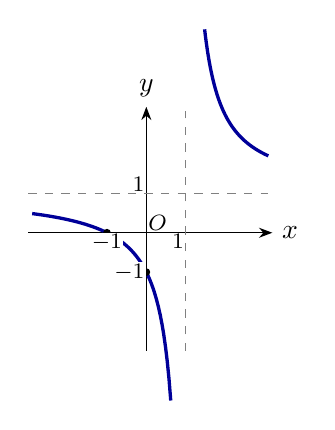
\begin{tikzpicture}[x=0.50cm,y=0.50cm,>=Stealth]
\draw[->] (-3.0,0)--(3.2,0) node[right] {$x$};
\draw[->] (0,-3.0)--(0,3.2) node[above] {$y$};
\draw[dashed,gray] (1,-3.0)--(1,3.1);
\draw[dashed,gray] (-3.0,1)--(3.1,1);
\draw[very thick,blue!60!black,domain=-2.9:0.62,samples=80] plot (\x,{(\x+1)/(\x-1)});
\draw[very thick,blue!60!black,domain=1.48:3.1,samples=80] plot (\x,{(\x+1)/(\x-1)});
\fill (0,-1) circle (1.4pt);\fill (-1,0) circle (1.4pt);
\node[above right,fill=white,inner sep=0.5pt] at (0,0) {\footnotesize $O$};
\node[below left,fill=white,inner sep=0.5pt] at (1,0) {\footnotesize $1$};
\node[above left,fill=white,inner sep=0.5pt] at (0,1) {\footnotesize $1$};
\node[below,fill=white,inner sep=0.5pt] at (-1,0) {\footnotesize $-1$};
\node[left,fill=white,inner sep=0.5pt] at (0,-1) {\footnotesize $-1$};
\end{tikzpicture}
\end{minipage}
\end{enumerate}

\newpage
\begin{enumerate}[start=7]
\item Một xưởng sản xuất ước tính chi phí trung bình (nghìn đồng) để sản xuất $x$ sản phẩm ($x>0$) là $\bar{C}(x)=\dfrac{2500}{x}+0{,}25x+40$. Xưởng cần sản xuất bao nhiêu sản phẩm để chi phí trung bình là thấp nhất?
\bonpa{$50$.}{$80$.}{$100$.}{$120$.}

\item Cho hình hộp $ABCD.A'B'C'D'$. Tổng vectơ $\vec{AB}+\vec{AD}+\vec{AA'}$ bằng vectơ nào dưới đây?
\bonpa{$\vec{AC}$.}{$\vec{BD'}$.}{$\vec{CA'}$.}{$\vec{AC'}$.}

\item Trong không gian $Oxyz$, cho hai điểm $A(2;-3;1)$ và $B(4;1;-5)$. Tọa độ trung điểm $M$ của đoạn thẳng $AB$ là
\bonpa{$(6;-2;-4)$.}{$(3;-1;-2)$.}{$(1;2;-3)$.}{$(2;4;-6)$.}

\item Trong không gian $Oxyz$, cho hai vectơ $\vec{a}=(1;-2;3)$ và $\vec{b}=(-2;1;1)$. Tọa độ của vectơ $\vec{u}=2\vec{a}+3\vec{b}$ là
\bonpa{$(-4;-1;9)$.}{$(4;1;-9)$.}{$(-1;-1;4)$.}{$(-4;1;9)$.}

\item Trong không gian $Oxyz$, cho hai vectơ $\vec{u}=(2;-1;1)$ và $\vec{v}=(1;3;-2)$. Tích vô hướng $\vec{u}\cdot\vec{v}$ bằng
\bonpa{$3$.}{$1$.}{$-3$.}{$-5$.}

\item Trong không gian $Oxyz$, cho hai điểm $A(1;2;-1)$ và $B(3;0;-2)$. Độ dài đoạn thẳng $AB$ bằng
\bonpa{$9$.}{$\sqrt{5}$.}{$\sqrt{13}$.}{$3$.}
\end{enumerate}

\vspace{3pt}
\section*{\large PHẦN II. Câu trắc nghiệm đúng hoặc sai}
\textit{Thí sinh trả lời từ câu 1 đến câu 4. Trong mỗi ý a), b), c), d) ở mỗi câu, thí sinh chọn đúng hoặc sai.}
\begin{enumerate}
\item Cho hàm số $y=f(x)=\dfrac{x^2-3x+3}{x-1}$.
\begin{enumerate}
\item Tập xác định của hàm số là $D=\mathbb{R}\setminus\{1\}$.
\item Đạo hàm của hàm số là $f'(x)=\dfrac{x^2-2x}{(x-1)^2}$.
\item Đồ thị hàm số có đường tiệm cận xiên là đường thẳng $y=x+2$.
\item Đồ thị hàm số có hai điểm cực trị $A$ và $B$. Độ dài đoạn thẳng $AB$ bằng $2\sqrt{5}$.
\end{enumerate}
\end{enumerate}

\newpage
\begin{enumerate}[start=2]
\item Một doanh nghiệp sản xuất một loại sản phẩm với số lượng $x$ trăm sản phẩm trong một đợt ($0\le x\le 80$). Tổng chi phí sản xuất (triệu đồng) được cho bởi hàm số $C(x)=x^3-60x^2+1500x+5000$. Doanh thu từ việc bán sản phẩm (triệu đồng) được cho bởi hàm số $R(x)=2700x-15x^2$. Lợi nhuận của doanh nghiệp là $P(x)=R(x)-C(x)$.
\begin{enumerate}
\item Chi phí cố định ban đầu của doanh nghiệp (khi chưa sản xuất sản phẩm nào) là $5000$ triệu đồng.
\item Doanh thu của doanh nghiệp khi bán được $20$ trăm sản phẩm là $48000$ triệu đồng.
\item Hàm lợi nhuận của doanh nghiệp là $P(x)=-x^3+45x^2+1200x-5000$.
\item Doanh nghiệp đạt lợi nhuận lớn nhất khi sản xuất $50$ trăm sản phẩm.
\end{enumerate}

\item Trong không gian $Oxyz$, cho ba điểm $A(1;2;0)$, $B(3;0;2)$ và $C(1;4;2)$.
\begin{enumerate}
\item Tọa độ của vectơ $\vec{AB}$ là $\vec{AB}=(2;-2;2)$.
\item Trọng tâm $G$ của tam giác $ABC$ có tọa độ là $G(2;2;1)$.
\item Tích vô hướng $\vec{AB}\cdot\vec{AC}=0$, suy ra tam giác $ABC$ vuông tại $A$.
\item Tọa độ điểm $D$ để tứ giác $ABCD$ là hình bình hành là $D(-1;6;0)$.
\end{enumerate}

\item Một chiếc đèn trang trí có trọng lượng $P=120\text{ N}$ được treo vào trần nhà bằng ba sợi dây cáp không dãn có độ dài bằng nhau, nối từ trần nhà tại ba điểm $A, B, C$ tới móc treo đèn $O$. Chọn hệ trục tọa độ $Oxyz$ có gốc tại $O$, tia $Oz$ hướng thẳng đứng lên trên. Khi đó trọng lực tác dụng lên đèn là $\vec{P}=(0;0;-120)$ (đơn vị: N). Lực căng của ba sợi dây tác dụng lên móc treo $O$ lần lượt là $\vec{T}_1, \vec{T}_2, \vec{T}_3$. Biết rằng ba lực $\vec{T}_1, \vec{T}_2, \vec{T}_3$ đôi một vuông góc và có cùng độ lớn $|\vec{T}_1|=|\vec{T}_2|=|\vec{T}_3|=T$.
\begin{enumerate}
\item Vì đèn ở trạng thái cân bằng nên $\vec{T}_1+\vec{T}_2+\vec{T}_3+\vec{P}=\vec{0}$.
\item Do ba lực $\vec{T}_1, \vec{T}_2, \vec{T}_3$ đôi một vuông góc nên $|\vec{T}_1+\vec{T}_2+\vec{T}_3|^2=|\vec{T}_1|^2+|\vec{T}_2|^2+|\vec{T}_3|^2=3T^2$.
\item Độ lớn của mỗi lực căng dây là $T=40\text{ N}$.
\item Góc $\alpha$ giữa mỗi sợi dây cáp và phương thẳng đứng thỏa mãn $\cos\alpha=\dfrac{\sqrt{3}}{3}$.
\end{enumerate}
\end{enumerate}

\vspace{3pt}
\section*{\large PHẦN III. Câu trắc nghiệm trả lời ngắn}
\textit{Thí sinh trả lời từ câu 1 đến câu 6. Mỗi câu trả lời đúng thí sinh được 0,5 điểm.}
\begin{enumerate}
\item Có bao nhiêu giá trị nguyên của tham số $m$ để hàm số $y=\dfrac{1}{3}x^3-mx^2+(m+2)x-2026$ đồng biến trên khoảng $(-\infty;+\infty)$?
\otraloi

\item Trong không gian $Oxyz$, cho hình hộp $ABCD.A'B'C'D'$ có $A(1;1;1)$, $B(2;3;4)$, $D(0;2;3)$ và $A'(2;0;5)$. Tìm tọa độ đỉnh $C'(x;y;z)$, sau đó tính tổng $S=x+y+z$.
\otraloi
\end{enumerate}

\newpage
\begin{enumerate}[start=3]
\item Cho hàm số $y=\dfrac{x^2+mx-2}{x-1}$. Biết rằng đồ thị hàm số có hai điểm cực trị nằm về hai phía của trục tung. Có bao nhiêu giá trị nguyên của tham số $m\in[-5;5]$ thỏa mãn yêu cầu bài toán?
\otraloi

\item Trong không gian $Oxyz$ (với đơn vị đo trên các trục là mét), có hai thiết bị bay không người lái (drone) $A$ và $B$ đang bay thử nghiệm. Tại thời điểm $t$ giây ($t\ge 0$), vị trí của drone $A$ là $A(t;2t;2)$ và vị trí của drone $B$ là $B(6-t;3;2+t)$. Khoảng cách ngắn nhất giữa hai drone trong quá trình bay bằng bao nhiêu mét?
\otraloi

\item Người ta muốn làm một chiếc hộp hình chữ nhật không nắp từ một tấm bìa carton hình chữ nhật có kích thước $80\text{ cm}\times 50\text{ cm}$ bằng cách cắt bỏ bốn hình vuông bằng nhau ở bốn góc (mỗi hình vuông có cạnh $x\text{ cm}$) rồi gấp các mép bìa lại (hình vẽ minh họa). Thể tích lớn nhất của chiếc hộp bằng bao nhiêu lít? (Biết $1\text{ lít}=1000\text{ cm}^3$).
\begin{center}
\begin{tikzpicture}[x=0.075cm,y=0.075cm,>=Stealth]
\fill[pattern=north east lines,pattern color=gray!80] (0,0) rectangle (10,10);
\fill[pattern=north east lines,pattern color=gray!80] (70,0) rectangle (80,10);
\fill[pattern=north east lines,pattern color=gray!80] (0,40) rectangle (10,50);
\fill[pattern=north east lines,pattern color=gray!80] (70,40) rectangle (80,50);
\draw[thick] (0,0) rectangle (80,50);
\draw[dashed,thick] (10,0)--(10,50) (70,0)--(70,50) (0,10)--(80,10) (0,40)--(80,40);
\draw[<->] (0,-4)--(80,-4) node[midway,fill=white,inner sep=1pt] {\small $80\text{ cm}$};
\draw[<->] (85,0)--(85,50) node[midway,right] {\small $50\text{ cm}$};
\draw[<->] (0,54)--(10,54) node[midway,above] {\small $x$};
\node[font=\small] at (40,25) {Phần bìa làm hộp};
\end{tikzpicture}
\par\smallskip{\footnotesize\textit{Hình minh họa, không theo tỉ lệ.}}
\end{center}
\otraloi

\item Một trạm cấp nước sạch $S$ nằm bên bờ một con sông thẳng cần dẫn nước đến một cụm dân cư $A$ ở bờ bên kia sông. Khoảng cách từ trạm cấp nước $S$ đến bờ sông đối diện là $SH=3\text{ km}$ ($H$ là hình chiếu vuông góc của $S$ lên bờ đối diện). Khoảng cách từ $H$ đến cụm dân cư $A$ dọc theo bờ sông là $HA=8\text{ km}$. Người ta dự định lắp đặt đường ống dẫn nước gồm hai đoạn: đoạn ống ngầm $SC$ đi dưới đáy sông từ $S$ đến điểm $C$ trên bờ sông đối diện (nằm giữa $H$ và $A$), và đoạn ống $CA$ chạy dọc theo bờ sông từ $C$ đến $A$. Biết chi phí lắp đặt mỗi kilômét đường ống ngầm dưới đáy sông là $100$ triệu đồng, chi phí lắp đặt mỗi kilômét đường ống trên bờ là $60$ triệu đồng. Tổng chi phí lắp đặt nhỏ nhất của toàn bộ đường ống bằng bao nhiêu triệu đồng?
\begin{center}
\begin{tikzpicture}[x=0.70cm,y=0.70cm,>=Stealth]
\draw[thick,blue!50!gray] (-0.5,2.0)--(8.5,2.0) node[right,black] {\footnotesize Bờ 1 (trạm $S$)};
\draw[thick,blue!50!gray] (-0.5,0)--(8.5,0) node[right,black] {\footnotesize Bờ 2};
\fill[cyan!10] (-0.5,0) rectangle (8.5,2.0);
\node at (4,1.0) {\textit{\footnotesize Sông}};
\coordinate (S) at (1,2.0);
\coordinate (H) at (1,0);
\coordinate (C) at (3.25,0);
\coordinate (A) at (7.8,0);
\fill (S) circle (2pt) node[above] {$S$};
\fill (H) circle (2pt) node[below] {$H$};
\fill (C) circle (2pt) node[below] {$C$};
\fill (A) circle (2pt) node[below] {$A$};
\draw[dashed] (S)--(H);
\draw (1,0.25)--(1.25,0.25)--(1.25,0);
\draw[line width=1.3pt,red!80!black] (S)--(C) node[midway,above,sloped] {\footnotesize ống ngầm};
\draw[line width=1.5pt,orange!80!black] (C)--(A) node[midway,above] {\footnotesize ống trên bờ};
\draw[<->] (0.4,0)--(0.4,2.0) node[midway,left] {\footnotesize $3\text{ km}$};
\draw[<->] (1,-0.55)--(7.8,-0.55) node[midway,below] {\footnotesize $8\text{ km}$};
\end{tikzpicture}
\par\smallskip{\footnotesize\textit{Hình minh họa sơ đồ lắp đặt đường ống nước.}}
\end{center}
\otraloi
\end{enumerate}
\begin{center}\textbf{---------------- HẾT ----------------}\end{center}

\newpage\pagestyle{answers}
\begin{center}\Large\textbf{BẢNG ĐÁP ÁN TỔNG HỢP}\end{center}
\textbf{Phần I. Trắc nghiệm nhiều phương án lựa chọn}
\begin{center}
\renewcommand{\arraystretch}{1.5}
\begin{tabular}{|c|*{12}{c|}}\hline
Câu & 1&2&3&4&5&6&7&8&9&10&11&12\\\hline
Đáp án & B & A & C & D & A & B & C & D & B & A & C & D \\\hline
\end{tabular}
\end{center}

\textbf{Phần II. Đúng hoặc sai}
\begin{center}
\renewcommand{\arraystretch}{1.4}
\begin{tabular}{|c|c|c|c|c|}\hline
Câu & a) & b) & c) & d)\\\hline
1 & Đ & Đ & S & Đ\\\hline
2 & Đ & Đ & Đ & S\\\hline
3 & Đ & S & Đ & Đ\\\hline
4 & Đ & Đ & S & Đ\\\hline
\end{tabular}
\end{center}

\textbf{Phần III. Trả lời ngắn}
\begin{center}
\renewcommand{\arraystretch}{1.5}
\begin{tabular}{|c|c|c|c|c|c|c|}\hline
Câu & 1 & 2 & 3 & 4 & 5 & 6\\\hline
Đáp án & 4 & 15 & 3 & 3 & 18 & 720 \\\hline
\end{tabular}
\end{center}

\textbf{Thang điểm dùng cho đề ôn tập:}
\begin{itemize}[leftmargin=*,itemsep=3pt]
\item Phần I: mỗi câu đúng $0{,}25$ điểm; tối đa $3$ điểm.
\item Phần II: mỗi câu có 4 ý. Đúng 1, 2, 3, 4 ý lần lượt được $0{,}1$; $0{,}25$; $0{,}5$; $1$ điểm. Tối đa $4$ điểm.
\item Phần III: mỗi câu đúng $0{,}5$ điểm; tối đa $3$ điểm.
\end{itemize}
\textbf{Phạm vi:} Bài 1–5 (ứng dụng đạo hàm và khảo sát hàm số), Bài 6–8 (vectơ và tọa độ trong không gian).
Tổng điểm $10$; thời gian $90$ phút.

\newpage
\begin{center}\Large\textbf{HƯỚNG DẪN GIẢI CHI TIẾT}\end{center}
\section*{\large Phần I}
\loigiai{Câu 1. Chọn B.}
Ta có $y'=-3x^2+6x=-3x(x-2)$.
Xét $y'>0\Leftrightarrow -3x(x-2)>0\Leftrightarrow 0<x<2$.
Vậy hàm số đã cho đồng biến trên khoảng $(0;2)$.

\loigiai{Câu 2. Chọn A.}
Ta có $y'=3x^2-12x+9=3(x-1)(x-3)$.
Phương trình $y'=0\Leftrightarrow x=1$ hoặc $x=3$.
Đạo hàm cấp hai: $y''=6x-12$.
Tại $x=1$, ta có $y''(1)=-6<0$, do đó $x=1$ là điểm cực đại của hàm số.

\loigiai{Câu 3. Chọn C.}
Tập xác định trên đoạn $[2;4]$ là $D=[2;4]$.
Đạo hàm: $f'(x)=\dfrac{2(x-1)-(2x+1)}{(x-1)^2}=\dfrac{-3}{(x-1)^2}<0,\ \forall x\in[2;4]$.
Do đó hàm số nghịch biến trên $[2;4]$, suy ra $\max_{[2;4]}f(x)=f(2)=\dfrac{2\cdot 2+1}{2-1}=5$.

\loigiai{Câu 4. Chọn D.}
Ta có $\lim_{x\to (-2)^+}\dfrac{3x-1}{x+2}=-\infty$ và $\lim_{x\to (-2)^-}\dfrac{3x-1}{x+2}=+\infty$ nên đường thẳng $x=-2$ là tiệm cận đứng.
Lại có $\lim_{x\to\pm\infty}\dfrac{3x-1}{x+2}=3$ nên đường thẳng $y=3$ là tiệm cận ngang.

\loigiai{Câu 5. Chọn A.}
Ta có $\dfrac{x^2-3x+4}{x-1}=x-2+\dfrac{2}{x-1}$.
Vì $\lim_{x\to\pm\infty}\left[\dfrac{x^2-3x+4}{x-1}-(x-2)\right]=\lim_{x\to\pm\infty}\dfrac{2}{x-1}=0$ nên đường tiệm cận xiên của đồ thị hàm số là đường thẳng $y=x-2$.

\loigiai{Câu 6. Chọn B.}
Dựa vào hình vẽ, đồ thị có đường tiệm cận đứng $x=1$ và tiệm cận ngang $y=1$.
Đồ thị đi qua điểm $(0;-1)$ và $(-1;0)$.
Trong các phương án đã cho, chỉ có hàm số $y=\dfrac{x+1}{x-1}$ thỏa mãn đầy đủ các điều kiện trên.

\loigiai{Câu 7. Chọn C.}
Xét hàm chi phí trung bình $\bar{C}(x)=\dfrac{2500}{x}+0{,}25x+40$ với $x>0$.
Đạo hàm: $\bar{C}'(x)=-\dfrac{2500}{x^2}+0{,}25$.
Cho $\bar{C}'(x)=0\Leftrightarrow x^2=\dfrac{2500}{0{,}25}=10000\Rightarrow x=100$ (do $x>0$).
Lập bảng biến thiên thấy hàm số đạt giá trị nhỏ nhất tại $x=100$.

\loigiai{Câu 8. Chọn D.}
Theo quy tắc hình hộp, với ba cạnh xuất phát từ cùng một đỉnh $A$ của hình hộp $ABCD.A'B'C'D'$, ta có $\vec{AB}+\vec{AD}+\vec{AA'}=\vec{AC'}$.

\loigiai{Câu 9. Chọn B.}
Tọa độ trung điểm $M$ của đoạn thẳng $AB$ là:
$x_M=\dfrac{2+4}{2}=3,\ y_M=\dfrac{-3+1}{2}=-1,\ z_M=\dfrac{1+(-5)}{2}=-2$.
Vậy $M(3;-1;-2)$.

\loigiai{Câu 10. Chọn A.}
Ta có $2\vec{a}=2(1;-2;3)=(2;-4;6)$ và $3\vec{b}=3(-2;1;1)=(-6;3;3)$.
Suy ra $\vec{u}=2\vec{a}+3\vec{b}=(2-6;-4+3;6+3)=(-4;-1;9)$.

\loigiai{Câu 11. Chọn C.}
Tích vô hướng của hai vectơ:
$\vec{u}\cdot\vec{v}=2\cdot 1+(-1)\cdot 3+1\cdot(-2)=2-3-2=-3$.

\loigiai{Câu 12. Chọn D.}
Ta có $\vec{AB}=(3-1;0-2;-2-(-1))=(2;-2;-1)$.\\
Độ dài đoạn thẳng $AB$ là $|\vec{AB}|=\sqrt{2^2+(-2)^2+(-1)^2}=\sqrt{9}=3$.

\newpage
\section*{\large Phần II}
\loigiai{Câu 1.}
a) Hàm số xác định khi mẫu số $x-1\ne 0\Leftrightarrow x\ne 1$. Do đó tập xác định $D=\mathbb{R}\setminus\{1\}$. Mệnh đề đúng.\\
b) Đạo hàm: $f'(x)=\dfrac{(2x-3)(x-1)-(x^2-3x+3)}{(x-1)^2}=\dfrac{2x^2-5x+3-x^2+3x-3}{(x-1)^2}=\dfrac{x^2-2x}{(x-1)^2}$. Mệnh đề đúng.\\
c) Thực hiện chia đa thức: $\dfrac{x^2-3x+3}{x-1}=x-2+\dfrac{1}{x-1}$.
Do $\lim_{x\to\pm\infty}[f(x)-(x-2)]=0$ nên đường tiệm cận xiên là $y=x-2$, chứ không phải $y=x+2$. Mệnh đề sai.\\
d) Cho $f'(x)=0\Leftrightarrow x(x-2)=0\Leftrightarrow x_1=0$ hoặc $x_2=2$.
Với $x=0\Rightarrow y=-3$, ta có cực trị $A(0;-3)$.
Với $x=2\Rightarrow y=1$, ta có cực trị $B(2;1)$.
Độ dài $AB=\sqrt{(2-0)^2+(1-(-3))^2}=\sqrt{4+16}=\sqrt{20}=2\sqrt{5}$. Mệnh đề đúng.

\loigiai{Câu 2.}
a) Chi phí cố định là chi phí khi $x=0$: $C(0)=5000$ (triệu đồng). Mệnh đề đúng.\\
b) Doanh thu khi bán $20$ trăm sản phẩm là: $R(20)=2700\cdot 20-15\cdot 20^2=54000-6000=48000$ (triệu đồng). Mệnh đề đúng.\\
c) Hàm lợi nhuận: $P(x)=R(x)-C(x)=(2700x-15x^2)-(x^3-60x^2+1500x+5000)=-x^3+45x^2+1200x-5000$. Mệnh đề đúng.\\
d) Đạo hàm hàm lợi nhuận: $P'(x)=-3x^2+90x+1200=-3(x^2-30x-400)=-3(x-40)(x+10)$.
Trên đoạn $[0;80]$, phương trình $P'(x)=0\Leftrightarrow x=40$.
Vì $P'(x)>0$ với $x\in(0;40)$ và $P'(x)<0$ với $x\in(40;80)$ nên lợi nhuận lớn nhất đạt được khi sản xuất $40$ trăm sản phẩm (tương ứng $4000$ sản phẩm). Mệnh đề sai.

\loigiai{Câu 3.}
a) Ta có $\vec{AB}=(3-1;0-2;2-0)=(2;-2;2)$. Mệnh đề đúng.\\
b) Tọa độ trọng tâm $G$ của tam giác $ABC$ là:
$x_G=\dfrac{1+3+1}{3}=\dfrac{5}{3},\ y_G=\dfrac{2+0+4}{3}=2,\ z_G=\dfrac{0+2+2}{3}=\dfrac{4}{3}$.
Tọa độ đúng là $G\left(\dfrac{5}{3};2;\dfrac{4}{3}\right)$, do đó mệnh đề sai.\\
c) Ta có $\vec{AC}=(1-1;4-2;2-0)=(0;2;2)$.
Tích vô hướng: $\vec{AB}\cdot\vec{AC}=2\cdot 0+(-2)\cdot 2+2\cdot 2=-4+4=0$.
Do đó $\vec{AB}\perp\vec{AC}$, suy ra tam giác $ABC$ vuông tại $A$. Mệnh đề đúng.\\
d) Tứ giác $ABCD$ là hình bình hành khi và chỉ khi $\vec{AD}=\vec{BC}$.
Ta có $\vec{BC}=(1-3;4-0;2-2)=(-2;4;0)$.
Gọi $D(x;y;z)$, ta có $\vec{AD}=(x-1;y-2;z-0)$.
Suy ra $\begin{cases}x-1=-2\\y-2=4\\z=0\end{cases}\Leftrightarrow\begin{cases}x=-1\\y=6\\z=0\end{cases}\Rightarrow D(-1;6;0)$. Mệnh đề đúng.

\loigiai{Câu 4.}
a) Khi chiếc đèn treo ở trạng thái cân bằng thì hợp lực của ba lực căng tác dụng lên móc treo phải triệt tiêu trọng lực của đèn, nghĩa là $\vec{T}_1+\vec{T}_2+\vec{T}_3+\vec{P}=\vec{0}$. Mệnh đề đúng.\\
b) Vì ba lực $\vec{T}_1, \vec{T}_2, \vec{T}_3$ đôi một vuông góc nên tích vô hướng từng đôi một bằng $0$:
$|\vec{T}_1+\vec{T}_2+\vec{T}_3|^2=|\vec{T}_1|^2+|\vec{T}_2|^2+|\vec{T}_3|^2+2(\vec{T}_1\cdot\vec{T}_2+\vec{T}_2\cdot\vec{T}_3+\vec{T}_3\cdot\vec{T}_1)=T^2+T^2+T^2=3T^2$. Mệnh đề đúng.\\
c) Từ câu a suy ra $\vec{T}_1+\vec{T}_2+\vec{T}_3=-\vec{P}$, do đó $|\vec{T}_1+\vec{T}_2+\vec{T}_3|=|\vec{P}|=120\text{ N}$.
Theo câu b, $3T^2=120^2=14400\Rightarrow T^2=4800\Rightarrow T=\sqrt{4800}=40\sqrt{3}\approx 69{,}28\text{ N}\ne 40\text{ N}$. Mệnh đề sai.\\
d) Đặt $\vec{T}=\vec{T}_1+\vec{T}_2+\vec{T}_3=-\vec{P}$, đây là vectơ có phương thẳng đứng hướng lên trên, độ lớn $|\vec{T}|=120\text{ N}=T\sqrt{3}$.
Góc $\alpha$ giữa sợi dây thứ nhất và phương thẳng đứng chính là góc giữa $\vec{T}_1$ và $\vec{T}$.
Ta có $\vec{T}\cdot\vec{T}_1=(\vec{T}_1+\vec{T}_2+\vec{T}_3)\cdot\vec{T}_1=|\vec{T}_1|^2=T^2$ (do $\vec{T}_2\cdot\vec{T}_1=\vec{T}_3\cdot\vec{T}_1=0$).
Mặt khác, $\vec{T}\cdot\vec{T}_1=|\vec{T}|\cdot|\vec{T}_1|\cdot\cos\alpha=T\sqrt{3}\cdot T\cdot\cos\alpha=T^2\sqrt{3}\cdot\cos\alpha$.
Suy ra $\cos\alpha=\dfrac{T^2}{T^2\sqrt{3}}=\dfrac{1}{\sqrt{3}}=\dfrac{\sqrt{3}}{3}$. Tương tự cho hai sợi dây còn lại. Mệnh đề đúng.

\newpage
\section*{\large Phần III}
\loigiai{Câu 1.}
Tập xác định $D=\mathbb{R}$. Đạo hàm: $y'=x^2-2mx+m+2$.
Hàm số đồng biến trên $(-\infty;+\infty)$ khi và chỉ khi $y'\ge 0,\ \forall x\in\mathbb{R}$.
Vì hệ số của $x^2$ là $a=1>0$, tam thức bậc hai không âm với mọi $x$ khi và chỉ khi:
$\Delta'\le 0\Leftrightarrow (-m)^2-(m+2)\le 0\Leftrightarrow m^2-m-2\le 0\Leftrightarrow -1\le m\le 2$.
Do $m\in\mathbb{Z}$ nên $m\in\{-1;0;1;2\}$.
Vậy có tất cả $4$ giá trị nguyên của tham số $m$ thỏa mãn.

\loigiai{Câu 2.}
Theo quy tắc hình hộp, ta có $\vec{AC'}=\vec{AB}+\vec{AD}+\vec{AA'}$.
Ta tính các vectơ:
$\vec{AB}=(2-1;3-1;4-1)=(1;2;3)$,
$\vec{AD}=(0-1;2-1;3-1)=(-1;1;2)$,
$\vec{AA'}=(2-1;0-1;5-1)=(1;-1;4)$.
Suy ra $\vec{AC'}=(1-1+1;2+1-1;3+2+4)=(1;2;9)$.
Tọa độ đỉnh $C'$ thỏa mãn $\vec{OC'}=\vec{OA}+\vec{AC'}=(1+1;1+2;1+9)=(2;3;10)$.
Vậy $C'(2;3;10)$, do đó tổng $S=x+y+z=2+3+10=15$.

\loigiai{Câu 3.}
Tập xác định $D=\mathbb{R}\setminus\{1\}$.
Đạo hàm: $y'=\dfrac{(2x+m)(x-1)-(x^2+mx-2)}{(x-1)^2}=\dfrac{x^2-2x+2-m}{(x-1)^2}$.
Đồ thị hàm số có hai điểm cực trị nằm về hai phía của trục tung khi và chỉ khi phương trình $g(x)=x^2-2x+2-m=0$ có hai nghiệm phân biệt $x_1, x_2$ khác $1$ và trái dấu nhau:
$\begin{cases}\Delta'=1-(2-m)=m-1>0\\ g(1)=1-2+2-m=1-m\ne 0\\ x_1 x_2=2-m<0\end{cases}\Leftrightarrow\begin{cases}m>1\\ m\ne 1\\ m>2\end{cases}\Leftrightarrow m>2$.
Kết hợp với điều kiện $m\in[-5;5]$ và $m\in\mathbb{Z}$, ta nhận các giá trị $m\in\{3;4;5\}$.
Vậy có $3$ giá trị nguyên thỏa mãn.

\loigiai{Câu 4.}
Tại thời điểm $t\ge 0$, vectơ nối vị trí hai drone là:
$\vec{AB}=(6-t-t;3-2t;2+t-2)=(6-2t;3-2t;t)$.
Bình phương khoảng cách giữa hai drone tại thời điểm $t$ là:
$d^2(t)=(6-2t)^2+(3-2t)^2+t^2=(36-24t+4t^2)+(9-12t+4t^2)+t^2=9t^2-36t+45$.
Biến đổi tam thức bậc hai:
$d^2(t)=9(t^2-4t+4)+9=9(t-2)^2+9\ge 9,\ \forall t\ge 0$.
Dấu đẳng thức xảy ra khi $t=2$ (thỏa mãn $t\ge 0$).
Vậy khoảng cách ngắn nhất giữa hai drone là $d_{\min}=\sqrt{9}=3\text{ mét}$.

\loigiai{Câu 5.}
Khi cắt bốn hình vuông cạnh $x\text{ (cm)}$ ở bốn góc thì điều kiện của $x$ là $0<x<25$.
Chiếc hộp tạo thành có kích thước ba chiều là:
Chiều dài đáy: $80-2x\text{ (cm)}$;
Chiều rộng đáy: $50-2x\text{ (cm)}$;
Chiều cao hộp: $x\text{ (cm)}$.
Thể tích của chiếc hộp là:
$V(x)=x(80-2x)(50-2x)=4x(40-x)(25-x)=4(x^3-65x^2+1000x)\text{ (cm}^3\text{)}$.
Đạo hàm: $V'(x)=4(3x^2-130x+1000)=4(x-10)(3x-100)$.
Trên khoảng $(0;25)$, phương trình $V'(x)=0$ có nghiệm duy nhất $x=10$.
Ta thấy $V'(x)>0$ khi $0<x<10$ và $V'(x)<0$ khi $10<x<25$, do đó thể tích hộp đạt giá trị lớn nhất tại $x=10\text{ cm}$.
Thể tích lớn nhất là:
$V(10)=10\cdot(80-20)\cdot(50-20)=10\cdot 60\cdot 30=18000\text{ cm}^3=18\text{ dm}^3=18\text{ lít}$.

\loigiai{Câu 6.}
Đặt độ dài đoạn $HC=x\text{ (km)}$ với $0\le x\le 8$.
Vì tam giác $SHC$ vuông tại $H$ nên độ dài đoạn ống ngầm dưới sông là:
$SC=\sqrt{SH^2+HC^2}=\sqrt{3^2+x^2}=\sqrt{x^2+9}\text{ (km)}$.
Độ dài đoạn ống dẫn chạy trên bờ sông từ $C$ đến $A$ là:
$CA=HA-HC=8-x\text{ (km)}$.
Tổng chi phí lắp đặt đường ống dẫn nước là hàm số theo $x$:
$f(x)=100\sqrt{x^2+9}+60(8-x)\quad (\text{triệu đồng})$.
Xét hàm số $f(x)$ trên đoạn $[0;8]$. Đạo hàm:
$f'(x)=\dfrac{100x}{\sqrt{x^2+9}}-60$.
Cho $f'(x)=0\Leftrightarrow \dfrac{100x}{\sqrt{x^2+9}}=60\Leftrightarrow \dfrac{5x}{\sqrt{x^2+9}}=3$
$\Leftrightarrow 25x^2=9(x^2+9)\Leftrightarrow 16x^2=81\Leftrightarrow x^2=\dfrac{81}{16}\Rightarrow x=\dfrac{9}{4}=2{,}25\text{ (do } x\ge 0\text{)}$.
Giá trị $x=2{,}25\in[0;8]$.
Ta tính giá trị của $f(x)$ tại các điểm biên và điểm dừng:
$f(0)=100\cdot 3+60\cdot 8=300+480=780\text{ triệu đồng}$;
$f(8)=100\cdot\sqrt{8^2+9}+60\cdot 0=100\sqrt{73}\approx 854{,}4\text{ triệu đồng}$;
$f(2{,}25)=100\cdot\sqrt{\left(\dfrac{9}{4}\right)^2+9}+60(8-2{,}25)=100\cdot\dfrac{15}{4}+60\cdot 5{,}75=375+345=720\text{ triệu đồng}$.
Vậy chi phí lắp đặt nhỏ nhất là $720$ triệu đồng (đạt được khi đặt trạm tiếp bờ $C$ cách $H$ một khoảng $2{,}25\text{ km}$).

\end{document}
